\section{Цель работы}
\begin{enumerate}
	\item Исследовать зависимость полной мощности, полезной мощности,
	      мощности потерь, падения напряжения во внешней цепи и КПД
	      источника от силы тока в цепи.
	\item Найти значения параметров источника: электродвижущей силы и
	      внутреннего сопротивления, оценить их погрешность.
\end{enumerate}

\section{Объект исследования}
Объект исследования --- ток в цепи.

\section{Метод экспериментального исследования}
Многократное прямое измерение характеристик тока в цепи

\section{Рабочие формулы и исходные данные}
\begin{enumerate}
	\item Полезная мощность $ P_R = U I $
	\item Полная мощность $P = \varepsilon I$
	\item Мощность потерь $P_S = I^2 r$
\end{enumerate}

\section{Измерительные приборы}
\begin{table}[ht]
	\centering
	\begin{tabular}{r l l r r}
    \toprule
    \textnumero{} п/п & Наименование & Тип прибора & Используемый диапазон           & Погрешность                       \\
    \midrule
		1               & Амперметр    & Цифровой    & 20 \unit{\milli\ampere}         & 0.01 \unit{\milli\ampere}         \\
		2               & Вольтметр    & Цифровой    & 20 \hspace{0.16cm} \unit{\volt} & 0.01 \hspace{0.16cm} \unit{\volt} \\
    \bottomrule
	\end{tabular}
	\caption{Измерительные приборы}
\end{table}

\section{Схема установки}
\begin{figure}[H]
	\centering
  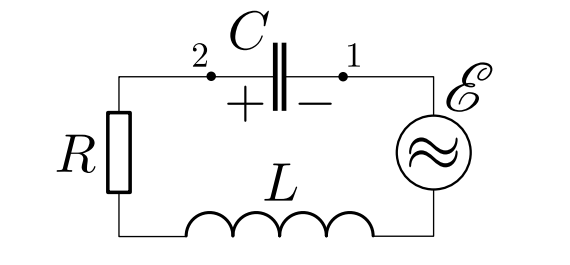
\includegraphics[width=0.9\textwidth]{./figures/scheme.png}
	\caption{Схема установки}
\end{figure}
